\chapter{Estudio de los componentes de la prótesis híbrida}\label{capitulo_2}
En el presente capítulo se va a explicar en mayor detalle cada uno de los componentes de la prótesis híbrida planteada en los objetivos del Trabajo Fin de Máster del capítulo introductorio.
\\
\\
Se pretende conocer en mayor profundidad cada componente y sus características en el estado que se encuentran al comienzo del presente trabajo, es decir, sin ningún tipo de modificación efectuada por el autor del mismo.
\\
\\
Terminada esta revisión y tras efectuar los cambios necesarios sobre cada componente de la prótesis a lo largo de los siguientes capítulos, se mostrará el montaje completo de la prótesis híbrida que se pretende construir.

\section{Electroestimulador muscular}
El electroestimulador utilizado en la prótesis híbrida ha sido desarrollado con anterioridad en el propio grupo de neurorrehabilitación del Insituto Cajal. Aparece en la figura \ref{fig:terefes} y se denomina mini TEREFES.\\

\begin{figure}[!htb]
\centering
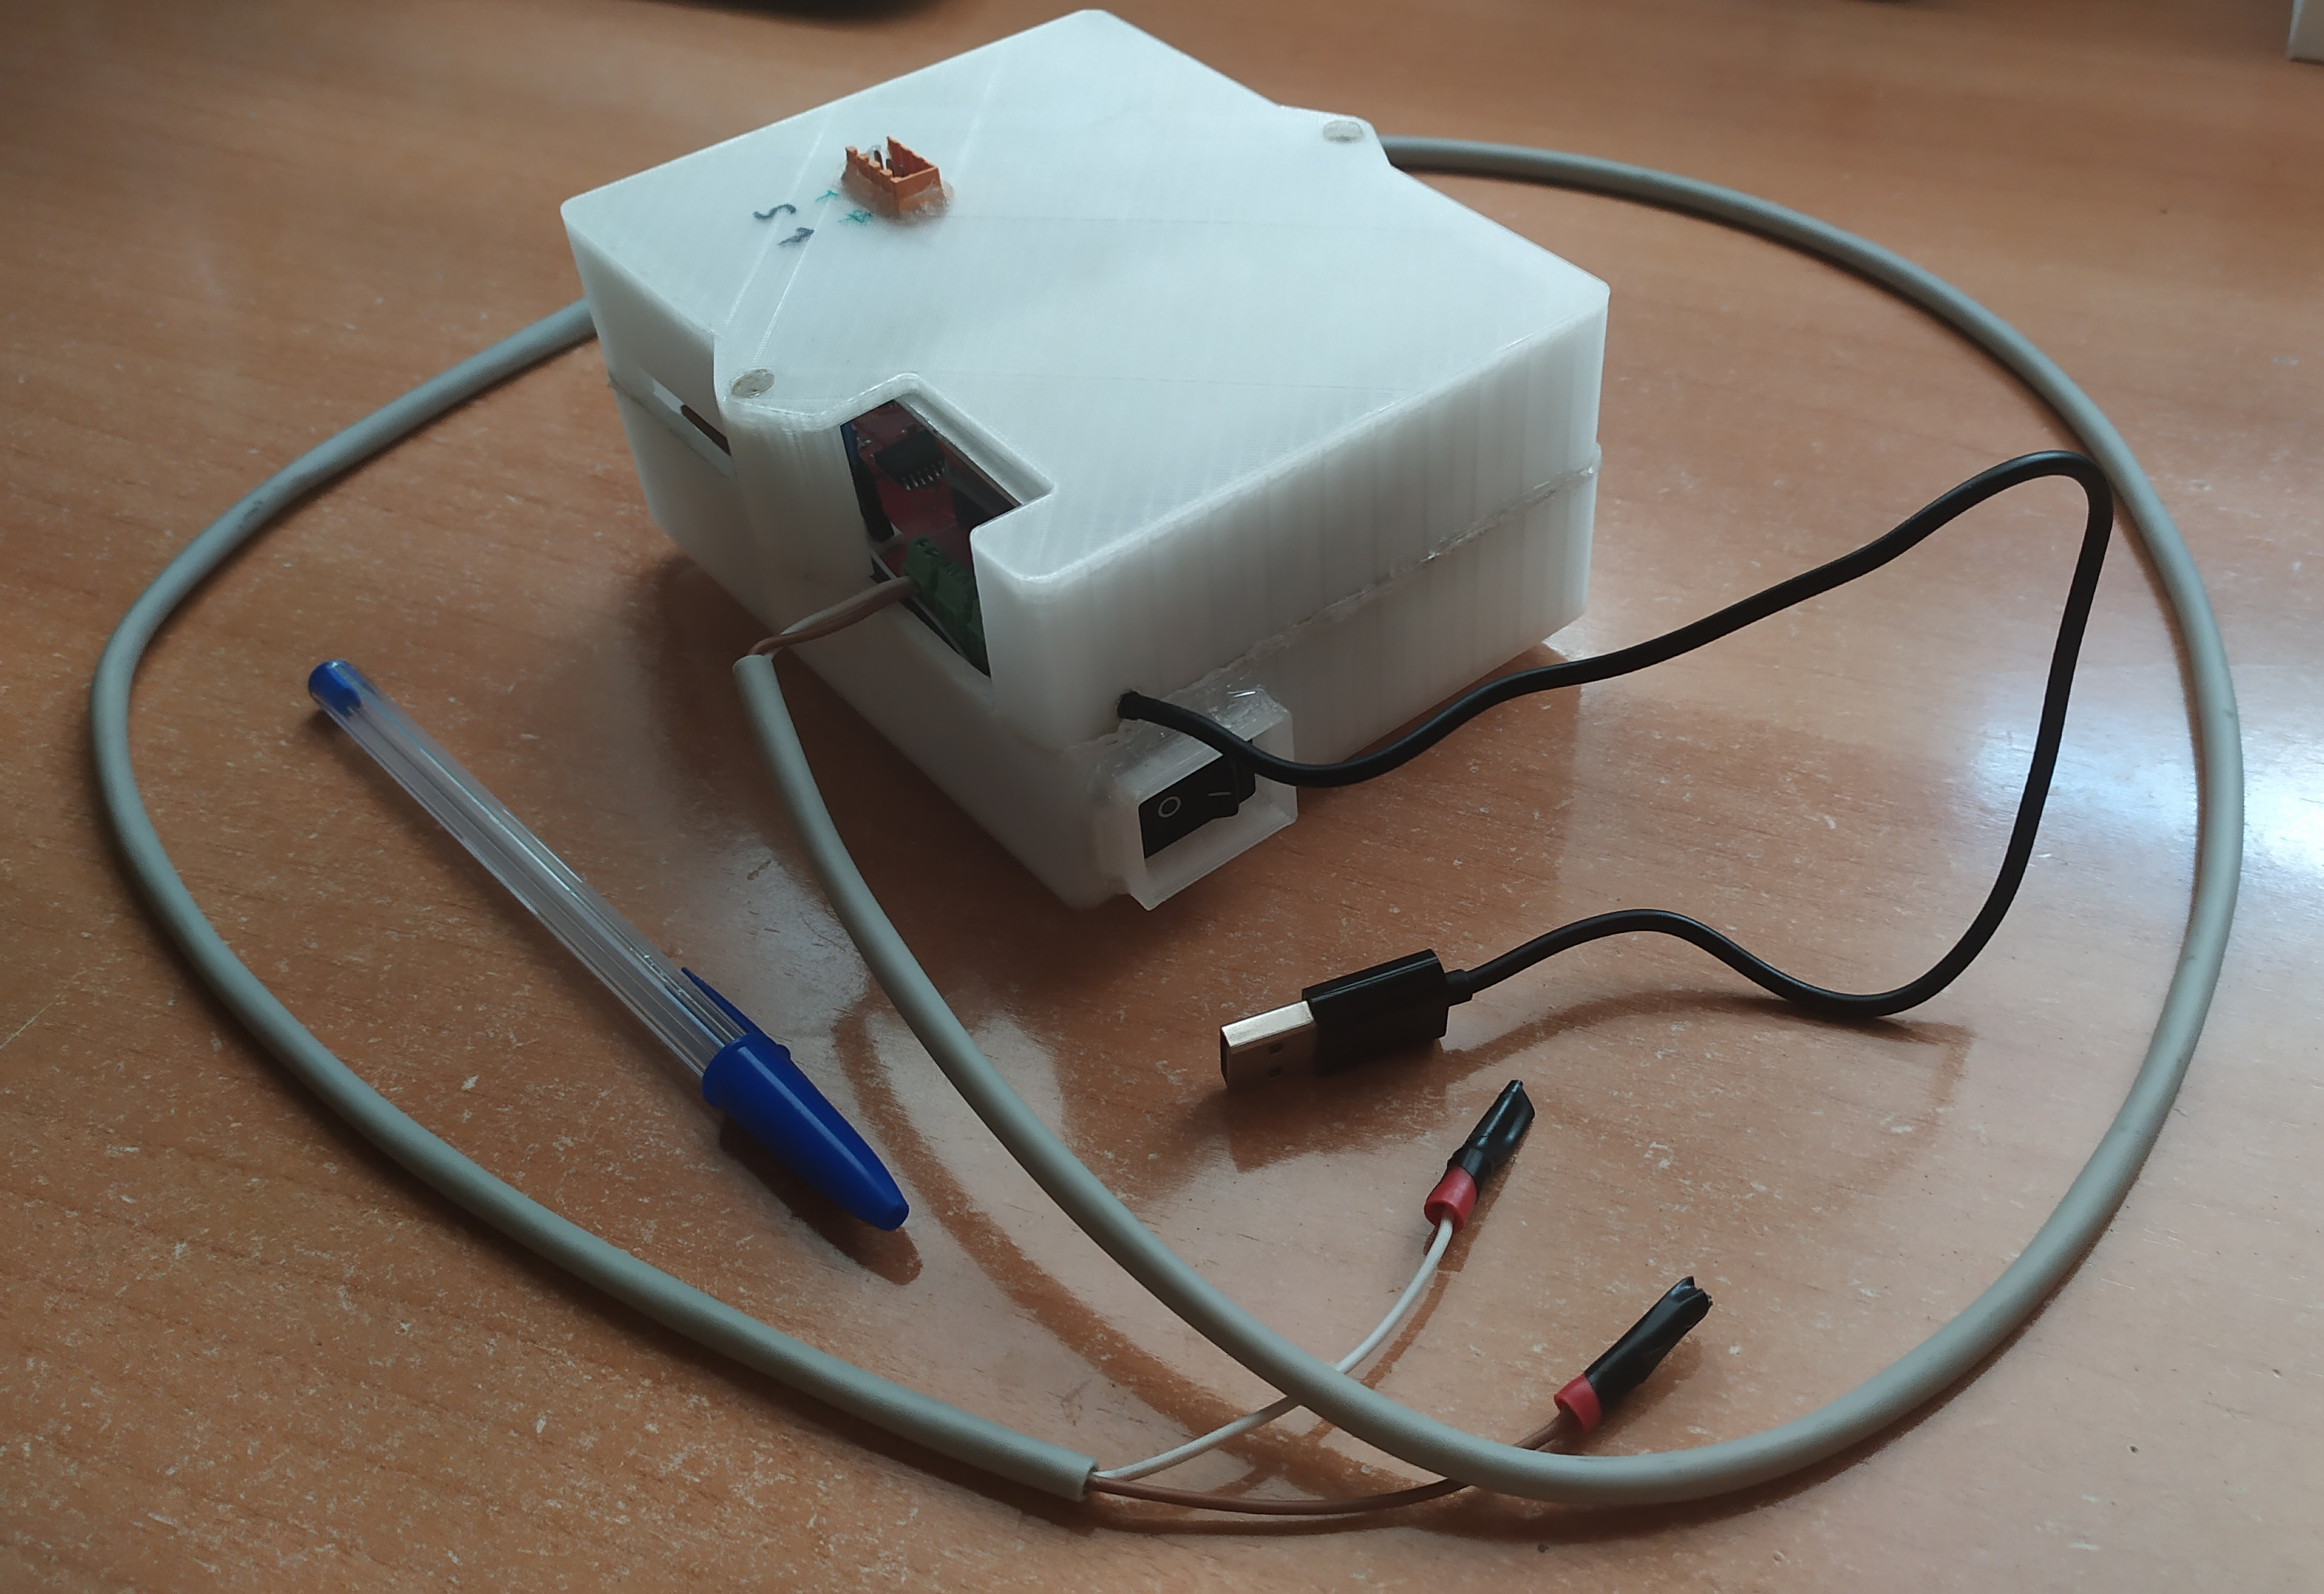
\includegraphics[scale=0.1]{terefes}
  \caption{Electroestimulador de 4 canales mini TEREFES. El cable negro USB tipo A permite la conexión a una fuente de 5V. El cable gris es la salida de uno de los canales con los extremos a los que iría el parche, sin conectar.}\label{fig:terefes}
\end{figure}

Este dispositivo dispone de 4 canales o salidas siendo cada una de ellas capaz de estimular un músculo o grupo de músculos. Esto lo hace mediante un par de electrodos conectados cada uno al estimulador con su respectivo cable. Se aprecian dichas salidas en la figura \ref{fig:canales}. Además, cada canal tiene su propia configuración de tren de pulsos de corriente, tal y como se ha explicado con anterioridad en los principios del funcionamiento de la electroestimulación. Se explicaron también una serie de parámetros de configuración del tren de pulsos de corriente y los cuales, para el caso del mini TEREFES, quedan recogidos en la tabla \ref{tabla:detalles_terefes}.\\


\begin{figure}[!htb]
\centering
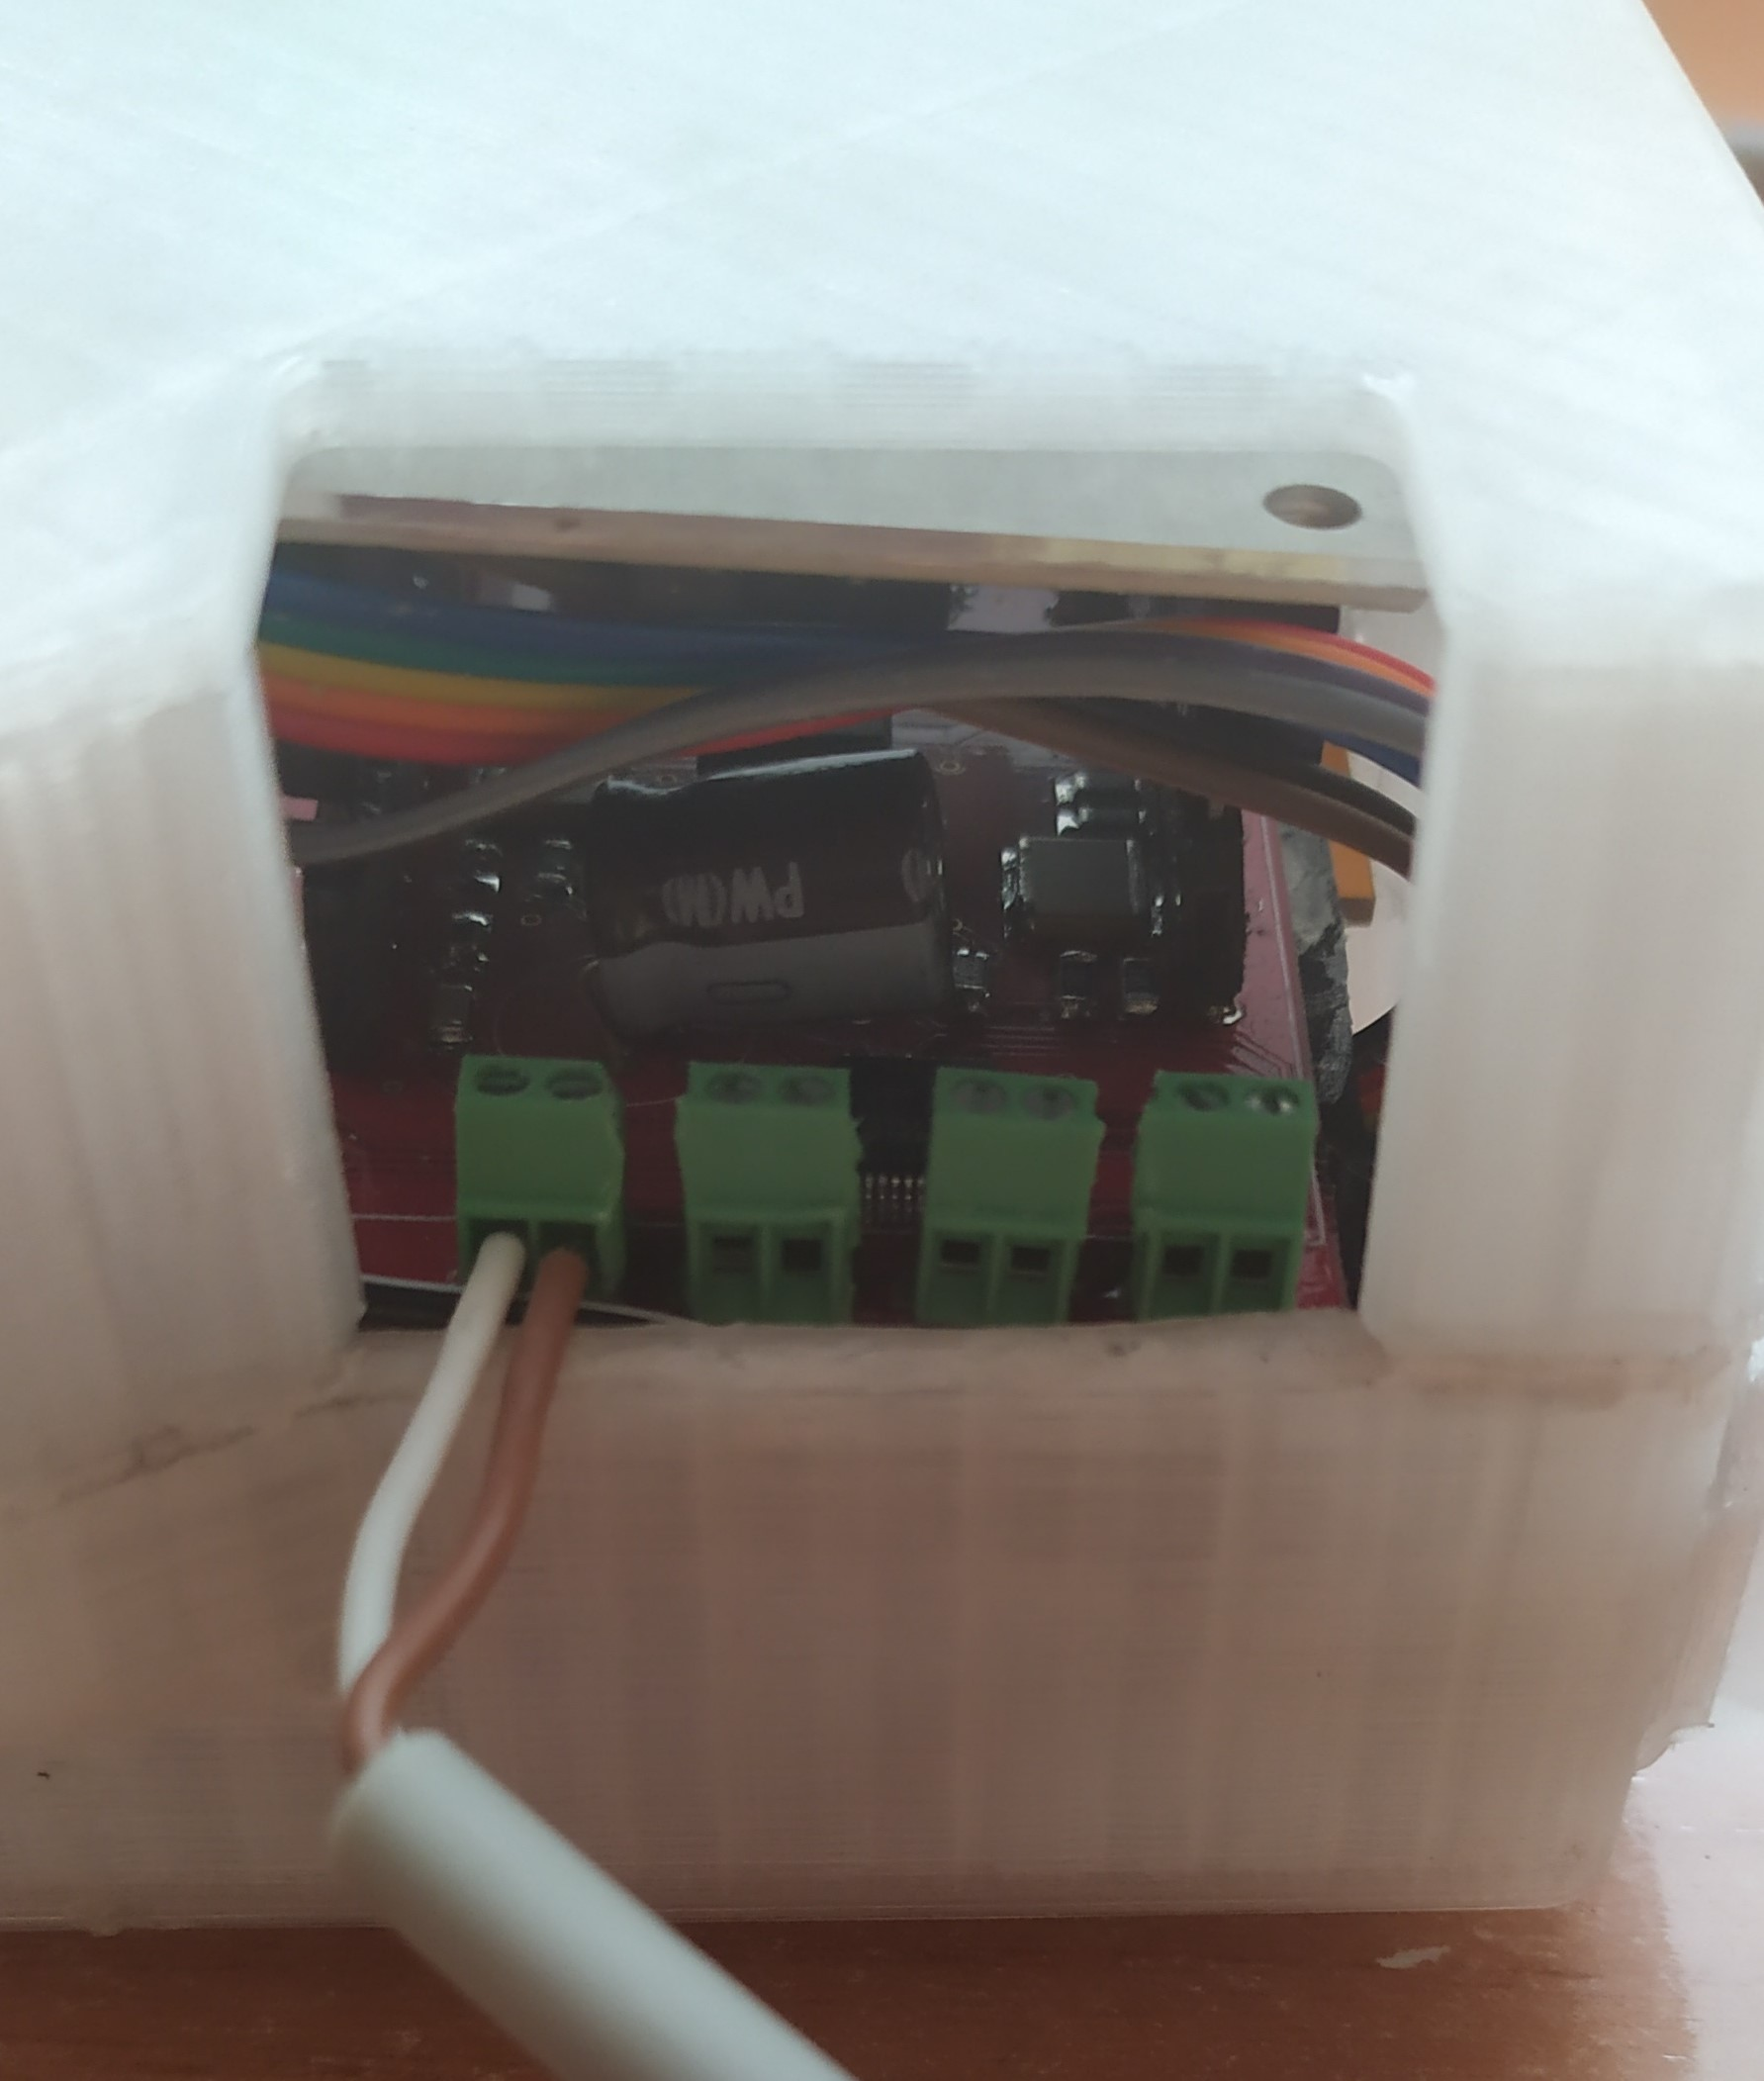
\includegraphics[scale=0.1]{canales}
  \caption{Conectores correspondientes a los 4 canales del estimulador.}\label{fig:canales}
\end{figure}

\begin{table}
\centering
\begin{tabular}{| p{30mm} | p{90 mm} |}
\hline
Corriente & De 0 a 90$mA$ en incrementos de 782.67$\mu A$ \\ \hline
Ancho de pulso & De 0 a 5000$\mu s$ en incrementos de 2.4$\mu s$\\ \hline
Frecuencia & Máximo de 100$Hz$ \\ \hline
Forma de pulso & Bifásico rectangular con tiempo interpulso de 100$\mu s$\\ \hline
Canales & Hasta 32 canales (dos módulos de 16 canales) de los que solamente se utilizan un máximo de 4\\ \hline
\end{tabular}\caption{Características del TEREFES.}\label{tabla:detalles_terefes}
\end{table}

El estimulador no dispone de batería interna por lo que es necesario alimentarlo a 5V mediante un cable USB tipo A. Para mayor portabilidad, y debido al voltaje y amperaje que maneja este dispositivo, cada estimulador dispone de una batería portátil de polímero de litio de $10000mAh$ y $5V$ a un máximo de $2.1A$ de descarga. Esta batería es similar a las utilizadas comúnmente para cargar teléfonos móviles y otros dispositivos de características parecidas.

\subsection{Hardware}
El hardware del electroestimulador tiene tres componentes principales:

\begin{itemize}
\item[•] Etapa de control
\item[•] Etapa de potencia
\item[•] Módulo de comunicación
\end{itemize}

\subsubsection{Etapa de control}
La etapa de control se encarga de la generación de la configuración de los trenes de pulsos de corriente para una correcta electroestimulación, aislamiento digital de estas señales y amplificación de las mismas. Sus principales componentes, en orden, desde la generación de la señal hasta su salida a los parches que se colocan en el paciente son:

\begin{itemize}
\item[1)] Un Microcontrolador Atmel de 8 bits y arquitectura AVR-RISC ATmega128L que genera las señales de configuración del tren de pulsos de corriente, entre otras funciones de control.
\item[2)] Cinco aisladores digitales alimentados por un regulador de tensión de 15 a 5 voltios y conectados a las señales generadas por el microcontrolador.
\item[3)] Un convertidor digital/analógico (DAC) de 8 bits junto a una referencia de tensión de 10V.
\item[4)] Primera etapa de amplificación de la salida del DAC con un amplificador operacional.
\item[5)] Segunda etapa de amplificación mediante un amplificador operacional de potencia con el cual se implementa una fuente de corriente tipo Howland mostrada en la figura \ref{fig:howland}. Se eligió utilizar este tipo de fuente de corriente por su linealidad en la ganancia de corriente, así como una reducida disminución de la corriente de salida ante impedancias elevadas en la carga\cite{FES}.\\

\begin{figure}[!htb]
\centering
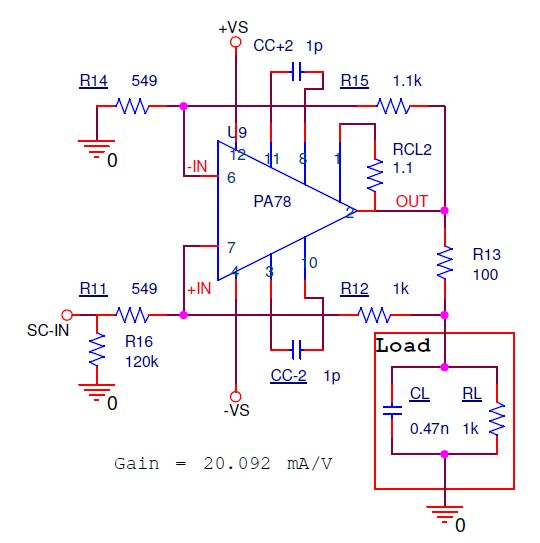
\includegraphics[scale=0.7]{howland}
  \caption{Fuente de corriente tipo Howland utilizada en el mini TEREFS\cite{FES}.}\label{fig:howland}
\end{figure}

\item[6)] Un switch analógico para controlar hasta cuatro canales o salidas, es decir, cuatro trenes de pulsos diferentes.
\end{itemize}

Se muestra en el Anexo I tanto el esquemático de esta etapa como la disposición de los componentes descritos en la tarjeta de circuito impreso.


\subsubsection{Etapa de potencia}\label{etapa_potencia}
La etapa de potencia se ha reciclado del TEREFES, estimulador del que procede el mini TEREFES. Esta se puede apreciar en el esquemático de la figura \ref{fig:fuente_terefes} y la cual está compuesta por dos fuentes de $\pm15VDC$ dos fuentes de $15VDC$ y una fuente de $5VDC$ que proporcionan dichos niveles de tensión a la etapa de control. Sin embargo, el mini TEREFES es un modelo más compacto y utiliza esta misma etapa de potencia pero prescindiendo de una de las fuentes de $15VDC$ y una de $\pm15VDC$ tal y como muestra el esquemático de la figura \ref{fig:fuente_mini_terefes}.\\

\begin{figure}[!htb]
\minipage{0.45\textwidth}
  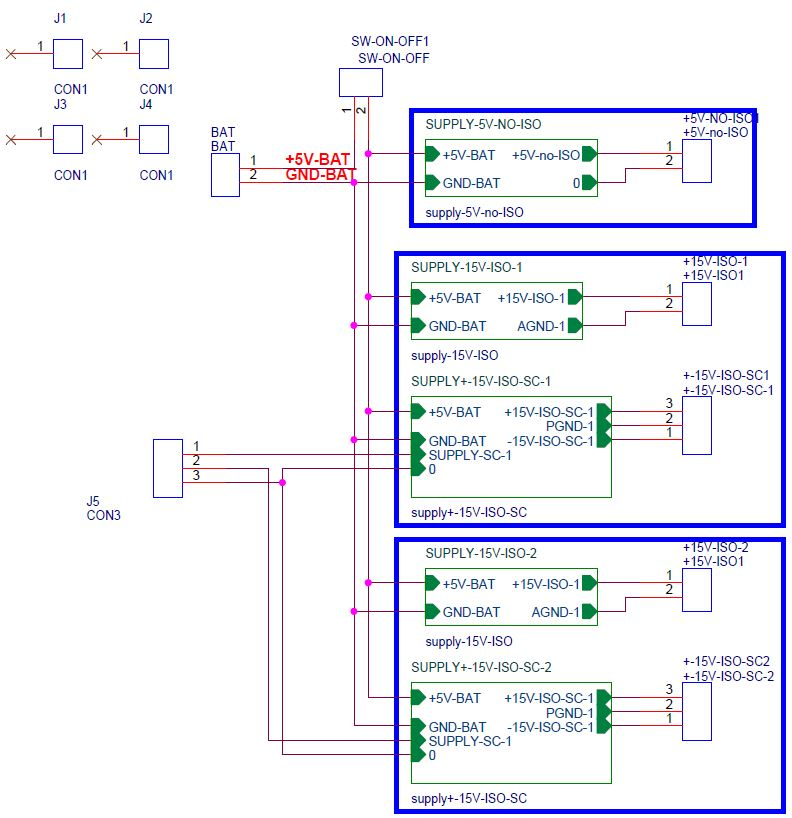
\includegraphics[width=\linewidth]{fuente_terefes}
  \caption{Esquemático de la etapa de potencia del TEREFES con alimentación a $5VDC$ de la batería (BAT), una fuente de $5VDC$ en cuadro el azul superior y dos fuentes de $15VDC$ y $\pm15VDC$, cada una de ellas en lod dos cuadros azules inferiores}\label{fig:fuente_terefes}
\endminipage\hfill
\minipage{0.45\textwidth}
  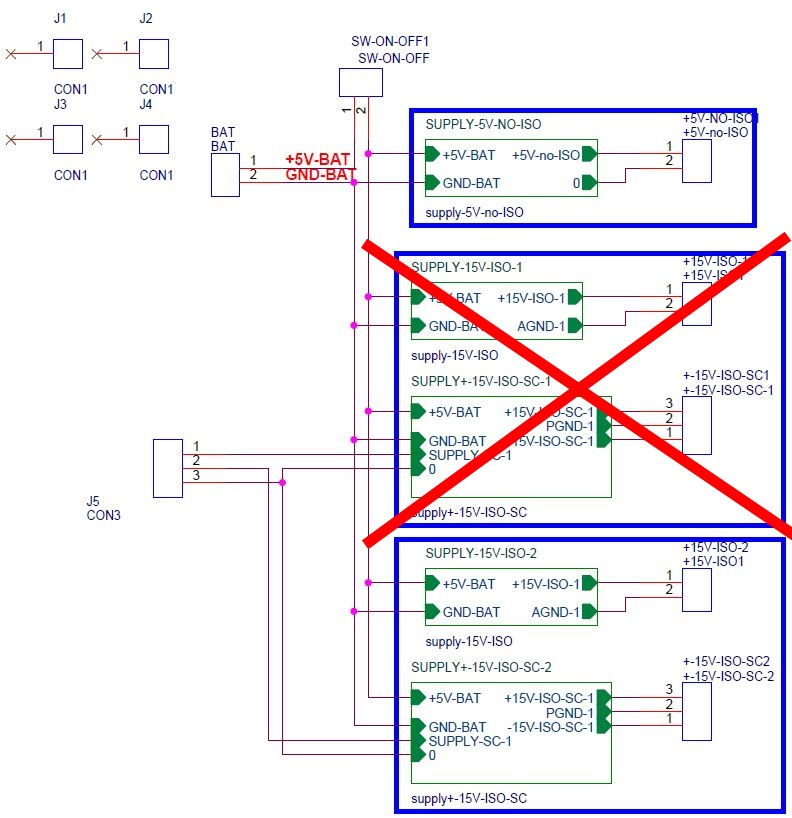
\includegraphics[width=\linewidth]{fuente_mini_terefes}
  \caption{Esquemático de la etapa de potencia del mini TEREFES con una fuente de $5VDC$ y otra de $15VDC$ y $\pm15VDC$}\label{fig:fuente_mini_terefes}
\endminipage\hfill
\end{figure}

La tarjeta de circuito impreso de la etapa de potencia recibe en su entrada $5VDC$ mediante el cable USB tipo A, tal y como se mencionó con anterioridad. Esta tensión alimenta a las fuentes de $5VDC$, $\pm15VDC$ y $15VDC$ las cuales están implementadas con los siguientes convertidores DC/DC:

\begin{itemize}
\item[•] Convertidor DC/DC de $5VDC$ a $5VDC$ a una corriente máxima de $400mA$.

\item[•] Convertidor DC/DC de $5VDC$ a $15VDC$ a una corriente máxima de $200mA$.

\item[•] Convertidor DC/DC de $5VDC$ a $\pm15VDC$ a una corriente máxima de $400mA$.
\end{itemize}

La etapa de potencia proporciona a la de control la alimentación a $5VDC$, $15VDC$ y $\pm15VDC$ utilizando los convertidores expuestos previamente. 

\subsubsection{Comunicación}
Existen dos formas de establecer comunicación con la etapa de control desde un dispositivo externo como puede ser un ordenador:

\begin{itemize}
\item[•] \textbf{Conexión In System Programming o ISP:} esta se usa para programar el microcontrolador mediante el conector ISP apreciable en el esquemático de la etapa de control en el Anexo I. Dado que el estimulador mini TEREFES utiliza un microcontrolador ATmega128L, que tiene arquitectura AVR-RISC, se hace uso del programador AVRISP mkII\cite{programador} para grabar el firmware. Dicho programador se puede ver en la figura \ref{fig:programador_micro}.

\item[•] \textbf{Interrupciones USART AVR:} se utilizan interrupciones para que el microcontrolador sea capaz de recibir y transmitir parámetros de configuración de la electroestimulación y otros datos. Para ello, se acopla al conector JP5 de la etapa de control el módulo Bluetooth Sparkfun Smirf Silver de la figura \ref{fig:modulo_bluetooth}. En dicho conector se tienen 4 pines: alimentación a 5V, pin de transmisión TX, pin de recepción RX y masa. De este modo, se establece conexión mediante un puerto serie virtual vía Bluetooth entre un ordenador y el módulo mencionado. Una vez establecida la conexión, el módulo Bluetooth sirve de intermediario entre el ordenador y el microcontrolador del estimulador para la transmisión de información. Se expondrán en mayor detalle todas las posibilidades de configuración en el apartado \ref{firmware}


%Otra forma de producir las interrupciones mencionadas y establecer comunicación entre un ordenador y el mini TEREFES es conectar mediante un cable un puerto USB del ordenador a los pines en los que se aloja el módulo Bluetooth. Sin embargo, es necesario utilizar un convertidor USB-USART, elemento no necesario si se utiliza el módulo Bluetooth pues éste ya hace esta conversión. Aún así, la velocidad de transmisión de datos siempre será superior en una conexión cableada frente a una inalámbrica. Se explorará esta opción en el capítulo correspondiente al estudio y mejora de la velocidad de transmisión de datos entre el microcontrolador y un dispositivo externo.

\end{itemize}

\begin{figure}[!htb]
\centering
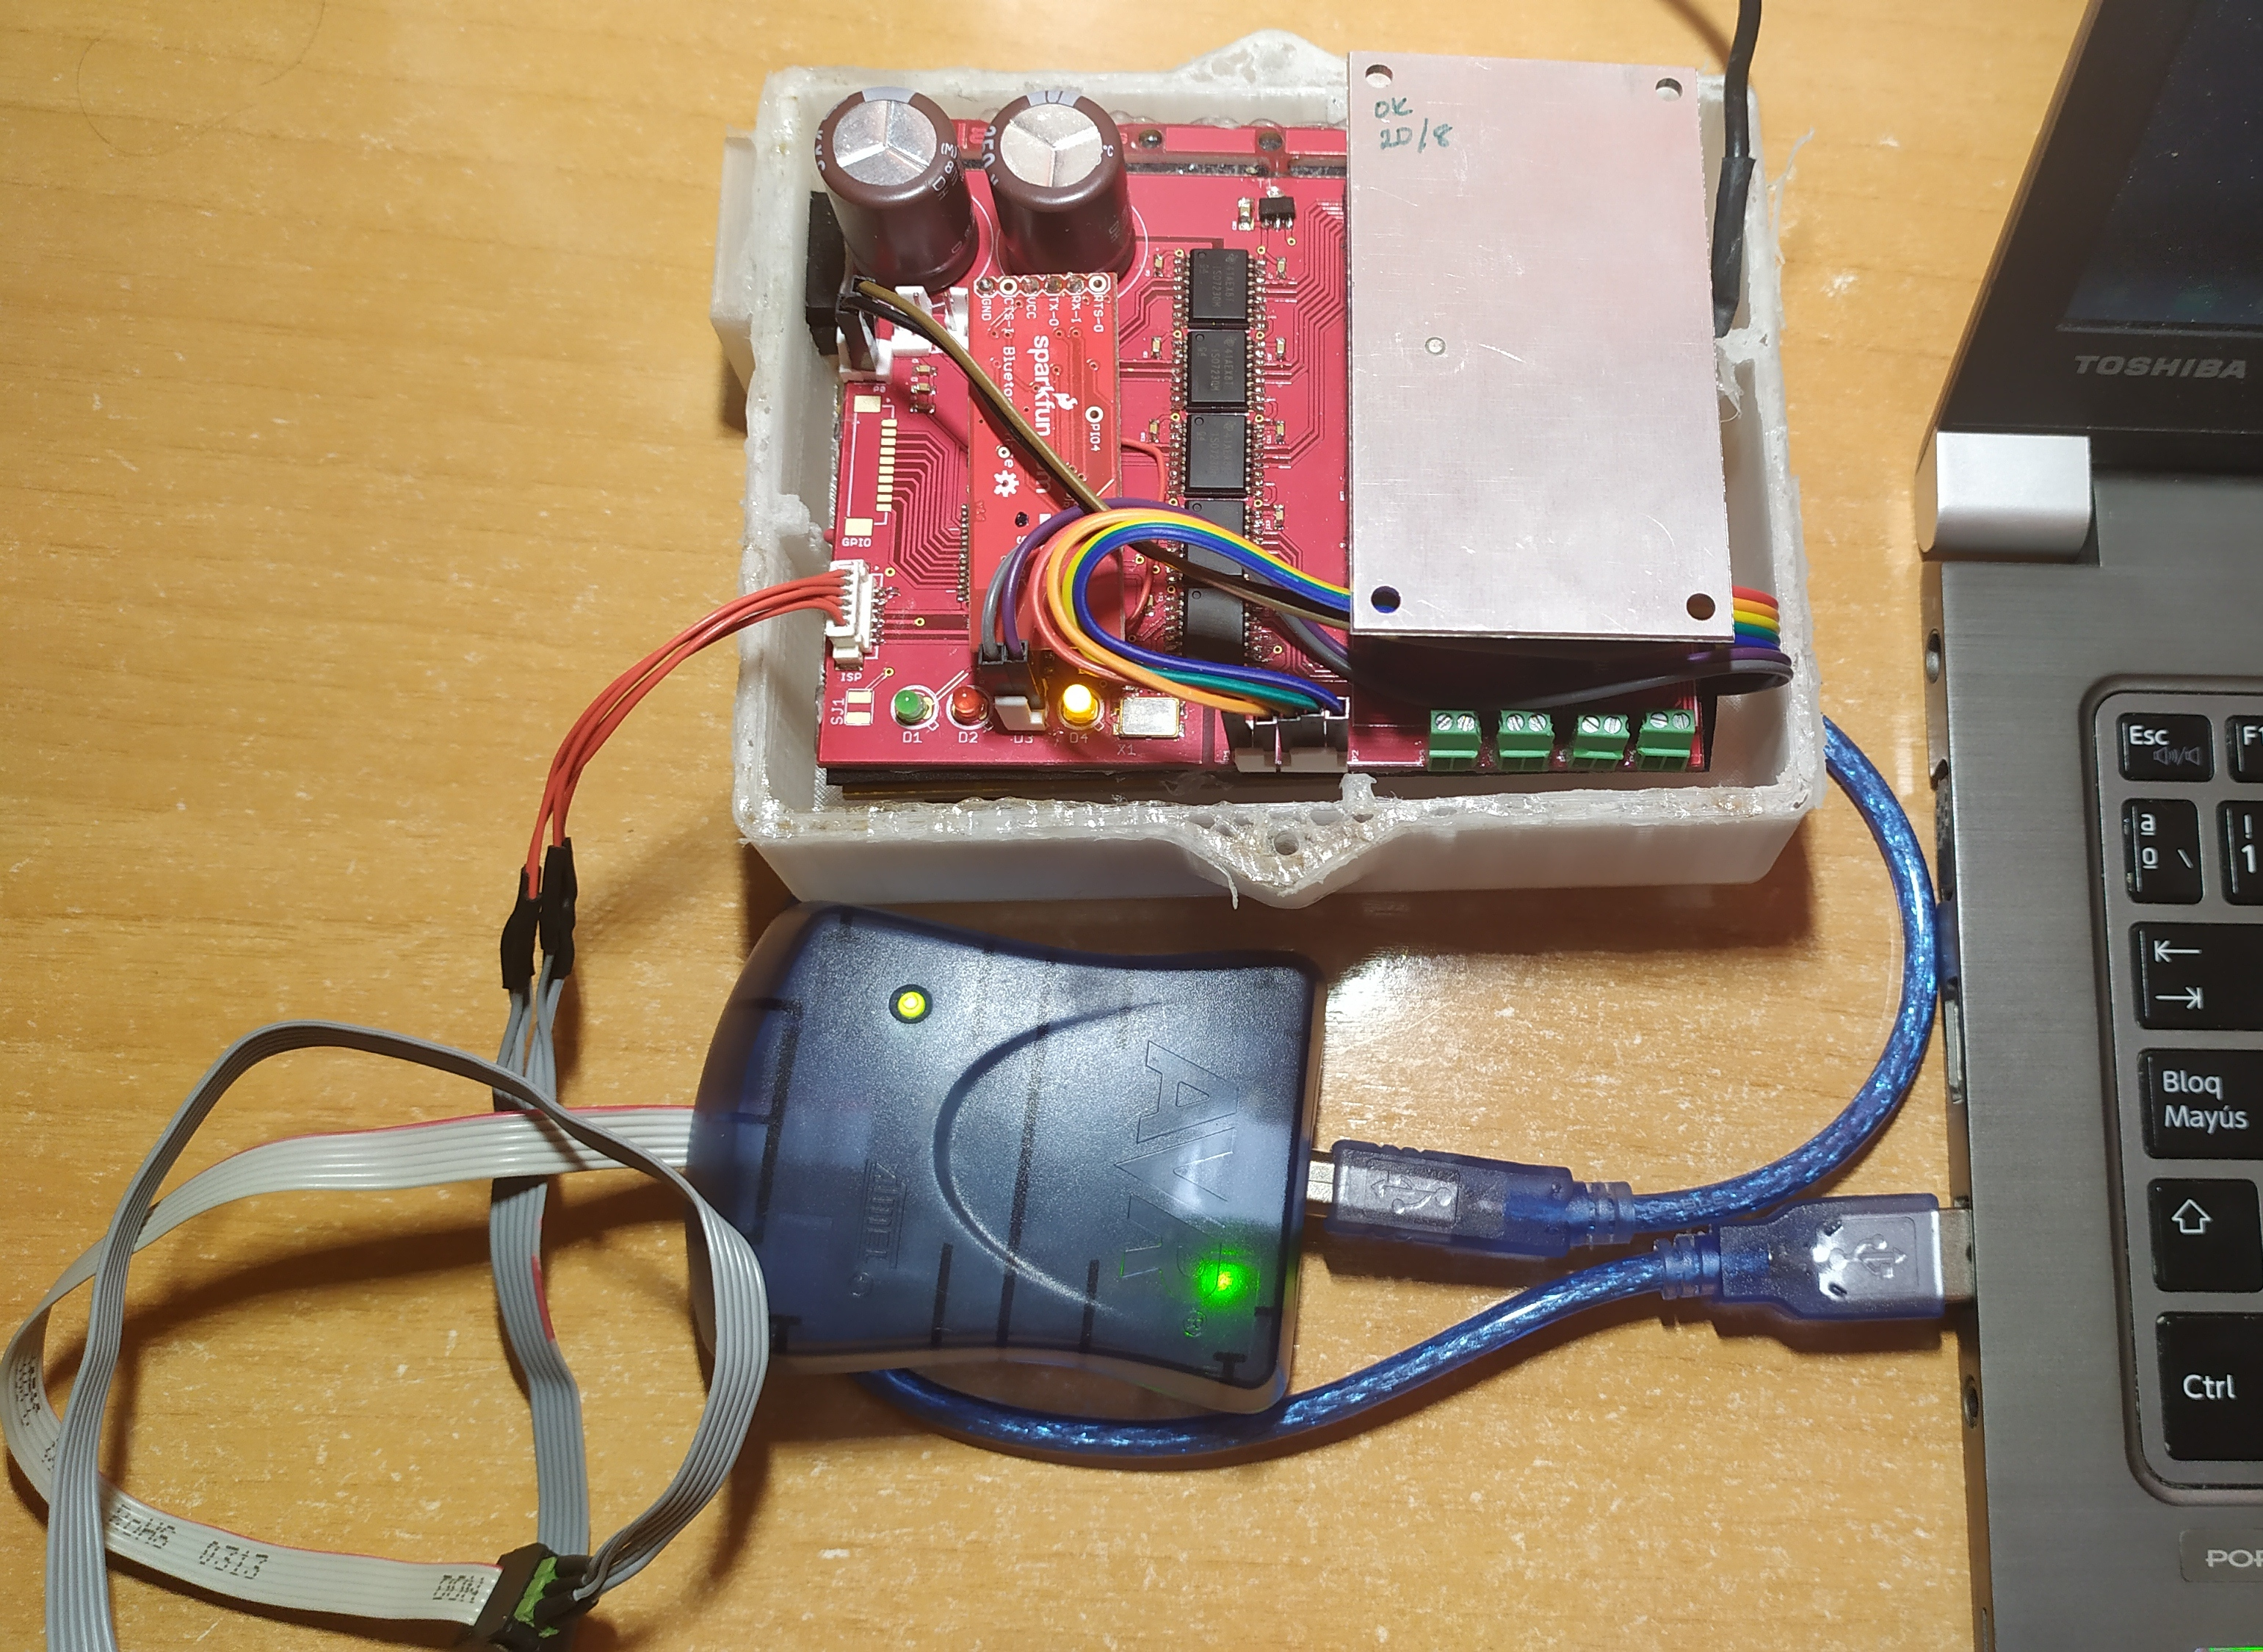
\includegraphics[scale=0.1]{programador_micro}
  \caption{Programador AVRISP mkII conectado al microcontrolador ATmega128 del mini TEREFES mediante ISP.}\label{fig:programador_micro}
\end{figure}

\begin{figure}[!htb]
\centering
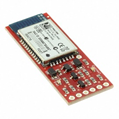
\includegraphics[scale=1.0]{modulo_bluetooth}
  \caption{Módulo Bluetooth Sparkfun Silver Smirf utilizado para la comunicación inalámbirca\cite{modulo_bluetooth}.}\label{fig:modulo_bluetooth}
\end{figure}

\subsection{Montaje}
La etapa de control recibe alimentación de la de potencia mediante los pines P0, P1 y P2 y que se pueden encontrar en su correspondiente esquemático en el Anexo I. En la figura \ref{fig:etapas} se muestra la conexión eléctrica entre las dos etapas del estimulador junto a la batería externa que lo alimenta. De este modo, los pines P0, P1 y P2 de la tarjeta de control que necesitan $5Vdc$, $15Vdc$ y $\pm15Vdc$ respectivamente, quedan unidos por cables a las fuentes de tensión correspondientes en la etapa de potencia.
\\
\\
En cuanto al montaje mecánico, apuntando a la reducción del tamaño del estimulador, sus dos etapas se colocaron enfrentadas por sus reversos separadas por espuma como elemento aislante. A continuación, se fijaron con adhesivo tal y como se aprecia en la figura \ref{fig:placas}.\\

\begin{figure}[!htb]
\minipage{0.5\textwidth}
  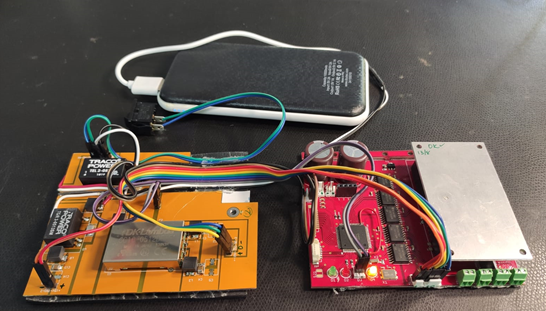
\includegraphics[width=\linewidth]{etapas}
  \caption{Etapas de control (placa roja) y de potencia (placa naranja) junto a la batería portátil que alimenta el estimulador. Los cables que conectan la placa de potencia con la de control proporcionan los niveles de tensión de $5VDC$, $15VDC$ y $\pm15Vdc$ explicados previamente.}\label{fig:etapas}
\endminipage\hfill
\minipage{0.4\textwidth}
  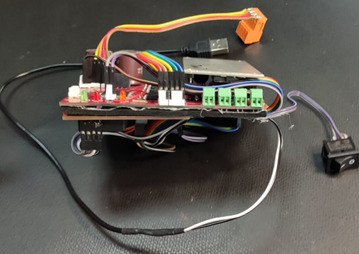
\includegraphics[width=\linewidth]{placas}
  \caption{Montaje de las etapas de control y potencia enfrentando los reversos de sus tarjetas de circuito impreso.}\label{fig:placas}
\endminipage\hfill
\end{figure}

Para contener todos los elementos anteriores se imprimió en 3D una caja para dicho propósito, la cual se muestra en la figura \ref{fig:montaje}. Se tiene además un elemento de sujección para que el estimulador esté fijado al paciente mediante un cinturón tal y como se ve en la figura \ref{fig:montaje_cinturon}.\\

\begin{figure}[!htb]
\centering
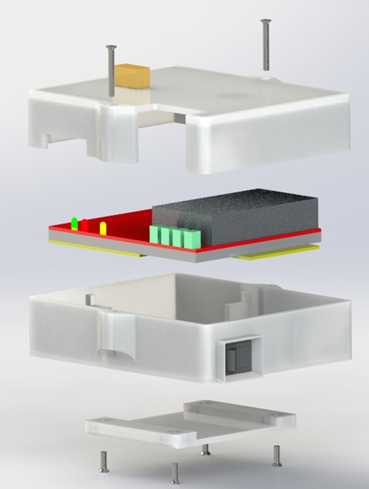
\includegraphics[scale=0.8]{montaje}
  \caption{Montaje del estimulador en la caja impresa en 3D. Desde arriba: tapa superior, etapas de control y potencia, tapa inferior con interruptor de encendido/apagado y elemento de sujección a un cinturón.}\label{fig:montaje}
\end{figure}


\subsection{Firmware}\label{firmware}
El firmware ha sido elaborado en la Universidad Católica de Asunción de Paraguay y permite el control y configuración de los parámetros de la electroestimulación, explicados en el capítulo \ref{capitulo_1} y de acuerdo a las especificaciones de la tabla \ref{tabla:detalles_terefes} mostrada con anterioridad.
\\
\\
Para el control de dichos parámetros, se debe entablar una comunicación entre el estimulador y un ordenador mediante puerto serie ya que se utiliza para enviar diferentes instrucciones. Debido a las capacidades de comunicación inalámbrica que posee el mini TEREFES, se puede establecer conexión con éste haciendo uso de cualquier ordenador que disponga de un módulo Bluetooth. Entonces, una vez completo el proceso de emparejar el dispositivo al ordenador mediante Bluetooth, se abre una terminal de puerto serie (por ejemplo Coolterm\cite{coolterm}) y se establece la conexión con el puerto asociado al estimulador habiendo establecido antes la siguiente configuración:

\begin{itemize}
\item[•] La velocidad de transmisión de datos debe ser de 115200 bits por segundo.
\item[•] La longitud de los mensajes es de 8 bits.
\item[•] Un bit de parada.
\item[•] Modo de paridad deshabilitado.
\item[•] Tras escribir un comando en la terminal, se pulsa la tecla ENTER para enviarlo, acción que el firmware debe detectar como un ``carriage return'' o retorno de carro. Por lo tanto, la acción del ENTER debe ser configurada en la terminal como retorno de carro y no como retorno de carro y nueva línea o line feed.
\end{itemize}

Una vez establecida la conexión, aparecerá en el terminal la línea ``NewCMD:'' devuelta por el dispositivo para indicar la solicitud de entrada de un nuevo comando por teclado. La figura \ref{fig:coolterm_conf} muestra la configuración del terminal descrita previamente.\\  

\begin{figure}[!htb]
\centering
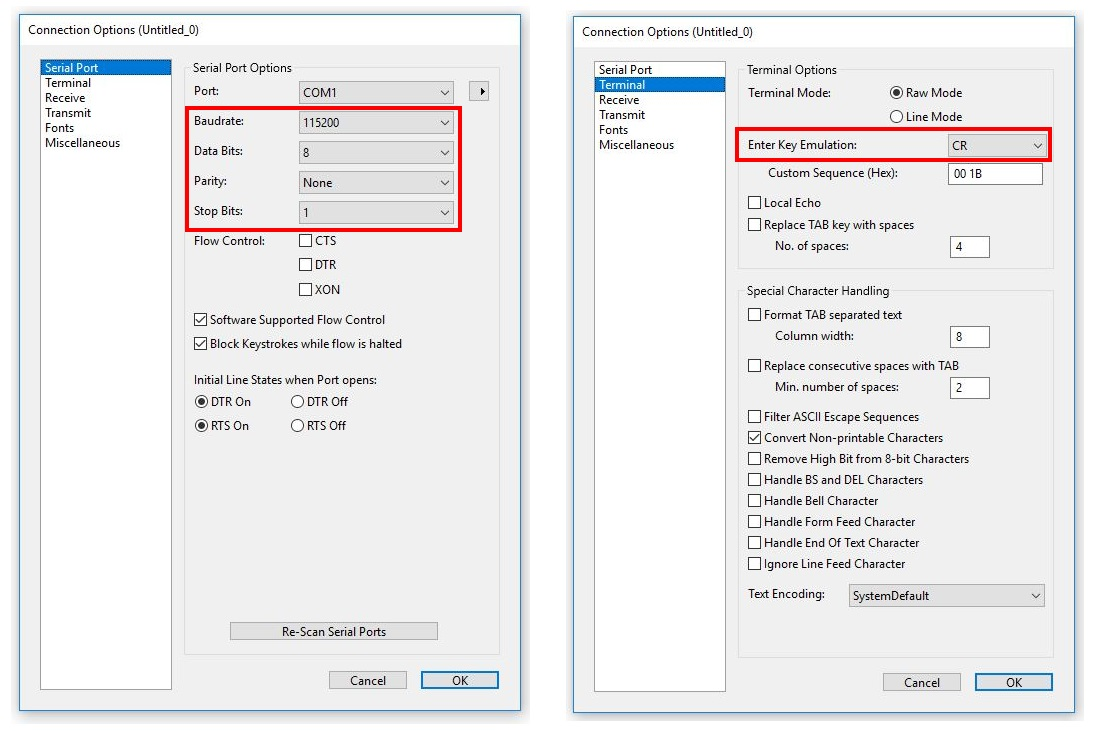
\includegraphics[scale=0.6]{coolterm_conf}
  \caption{Configuración del terminal.}\label{fig:coolterm_conf}
\end{figure}


Para el control del estimulador mediante instrucciones, se ha de considerar en primer lugar si se van a utilizar dos o más canales de estimulación. Si es el caso, se deben configurar los siguientes parámetros que pueden considerarse como los parámetros generales del estimulador:

\begin{itemize}
\item[•] \textbf{Número de canales (fl):} indica el número de canales que debe utilizar el estimulador.
\item[•] \textbf{Lista de canales (lc):} establece el orden de estimulación de los canales, es decir, qué turno tiene cada canal a la hora de estimular ya que un mismo dispositivo no activa dos o más canales a la vez. 
\item[•] \textbf{Frecuencia inter grupo (tg):} indica la frecuencia de repetición de un patrón de estimulación de canales. Debe introducirse en Hz.
\item[•] \textbf{Frecuencia intra grupo (ti):} indica la frecuencia de repetición de la estimulación de un canal dentro de un patrón de estimulación de canales. Debe introducirse en Hz, es decir. La figura \ref{fig:parametros_generales} muestra las frecuencias mencionados.
\end{itemize}

Para configurar o escribir un valor en los parámetros descritos se introduce un comando de la siguiente forma:
$$e\;fl\;[número\;de\;canales\;0-3]$$
$$e\;lc\;[número\;de\;canal\;0-3]\;[turno\;0-3]$$
$$e\;tg\;[frecuencia\;0-255]$$
$$e\;ti\;[frecuencia\;0-255]$$

Se indica entre corchetes el tipo y rango de valores numéricos que debe introducir el usuario por teclado destacando que los valores comienzan en cero y no en uno. Por ejemplo, si se desea utilizar 2 canales siendo el canal 1 el primero en estimular y el canal 2 el segundo en estimular se debe escribir en la terminal:
$$e\;fl\;1$$
$$e\;lc\;0\;0$$
$$e\;lc\;1\;1$$

También es posible leer en el terminal el valor que tienen estos parámetros en el estimulador. Para ello, se deben enviar los siguientes comandos al estimulador para solicitar que transmita el valor de los parámetros especificados:
$$l\;fl$$
$$l\;lc$$
$$l\;tg$$
$$l\;ti$$

\begin{figure}[!htb]
\centering
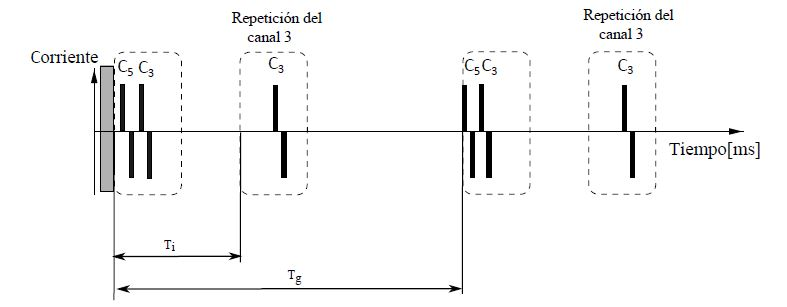
\includegraphics[scale=0.8]{parametros_generales}
  \caption{Frecuencias inter (tg) e intra (ti) grupo sobre un tren de pulsos de corriente. Se muestran en la figura como periodos pero el estimulador trabaja con su inverso, es decir, frecuencia.}\label{fig:parametros_generales}
\end{figure}

Por otra parte, cada canal admite las siguientes configuraciones de parámetros y que pueden quedar definidos como los parámetros de canal:

\begin{itemize}
\item[•] \textbf{Amplitud de corriente:} la amplitud de corriente eléctrica tanto para pulsos positivos (ap) como negativos (an).
\item[•] \textbf{Ancho de pulso:} duración del pulso de corriente positiva (tp) y negativa (tn).
\item[•] \textbf{Repeticiones (re):} repeticiones de estimulación de un canal dentro de un tren de pulsos.
\item[•] \textbf{Inversión de pulso (in):} determina si el primer pulso es positivo o negativo.
\end{itemize}

Para configurar los valores de dichos parámetros se debe introducir el comando correspondiente de la forma:

$$w\;[número\;de\;canal\;0-3]\;ap/an\;[amplitud\;0-115]$$
$$w\;[número\;de\;canal\;0-3]\;tp/tn\;[amplitud\;0-2100]$$
$$w\;[número\;de\;canal\;0-3]\;re\;[repeticiones\;0-3]$$
$$w\;[número\;de\;canal\;0-3]\;in\;[inversión\;0-1]$$

En el primer y segundo comando se debe elegir ap o an. Los valores de inversión de pulso son 0 si se quiere mantener el primer pulso positivo o 1 si se quiere invertir, es decir que el primer pulso sea de corriente negativa.
\\
\\
Por el contrario, si se desea leer todos estos valores asociados a un canal se debe introducir:
$$r\;[número\;de\;canal\;0-3]$$

Por último, existen los siguientes comandos de control:

\begin{itemize}
\item[•] \textbf{Encendido/apagado de tensión de $\pm15Vdc$}. Se ha implementado esta característica para reducir el consumo del electroestimulador. El comando para encender la fuente es $on1$ y para apagarla $off1$.
\item[•] \textbf{Comienzo/detención de la estimulación.} Para comenzar la estimulación se introduce el comando $s$ y para detenerla el comando $p$.
\item[•] \textbf{Modo de operación}. Existen hasta seis modos diferentes en los que puede operar el estimulador. Principalmente determinan cómo se produce la estimulación ya sea de forma continuada, interrumpida y otras variantes para las que no se entrará en más detalle. Se configura un modo de operación con un comando de la forma $e\;md\;[número\;de\;modo\;1-6]$. Si se desea leer el modo configurado se escribe $l\;md$
\item[•] \textbf{Guardado de parámetros.} Mediante el comando $g$ se pueden guardar en la EEPROM del microcontrolador del todos los valores configurados previamente.
\end{itemize}

Se muestra en la figura \ref{fig:coolterm_ejemplo} un ejemplo del control del estimulador en coolterm mediante las instrucciones descritas.\\

\begin{figure}[!htb]
\centering
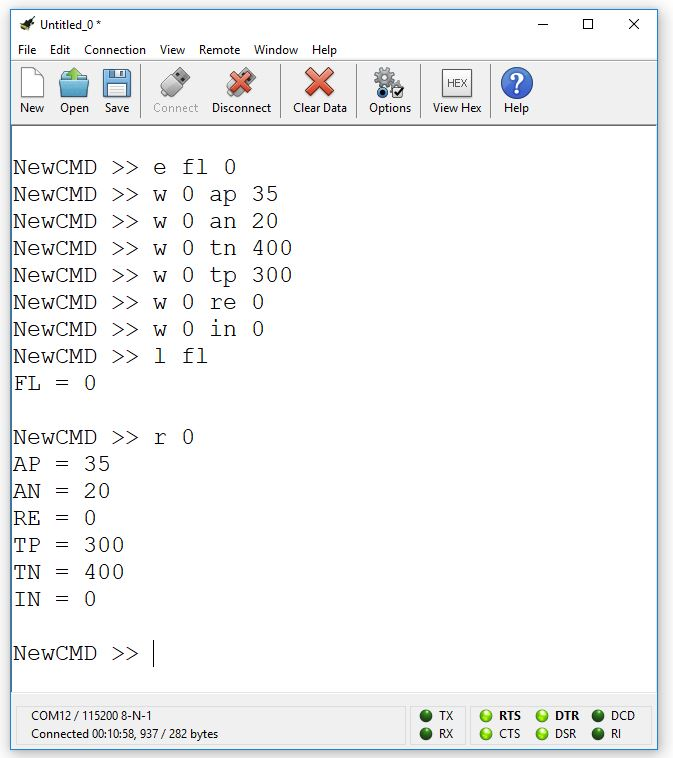
\includegraphics[scale=0.5]{coolterm_ejemplo}
  \caption{Ejemplo de utilización de instrucciones sobre el estimulador eléctrico mediante coolterm.}\label{fig:coolterm_ejemplo}
\end{figure}

Cabe destacar que los valores numéricos correspondientes a los parámetros de corriente (ap y an) ancho de pulso (tp y tn) y frecuencia (tg y ti) no son los reales o físicos, es decir, no son unidades de corriente, tiempo ni frecuencia. Para traducir estos valores a sus correspondientes magnitudes físicas se hace una conversión interna en el estimulador mediante los correspondientes factores de conversión obtenidos empíricamente. Se aprecia en la figura \ref{fig:factores_corriente_ancho} que la relación entre el valor manejado por el estimulador y las magnitudes físicas de intensidad de corriente y ancho de pulso se pueden considerar lineales, por lo que el factor de conversión será una constante. Sin embargo, esto no ocurre con el parámetro de frecuencia cuya función de conversión ha sido deducida tal y como se ve en la figura \ref{fig:factor_frecuencia}.\\

\begin{figure}[!htb]
\centering
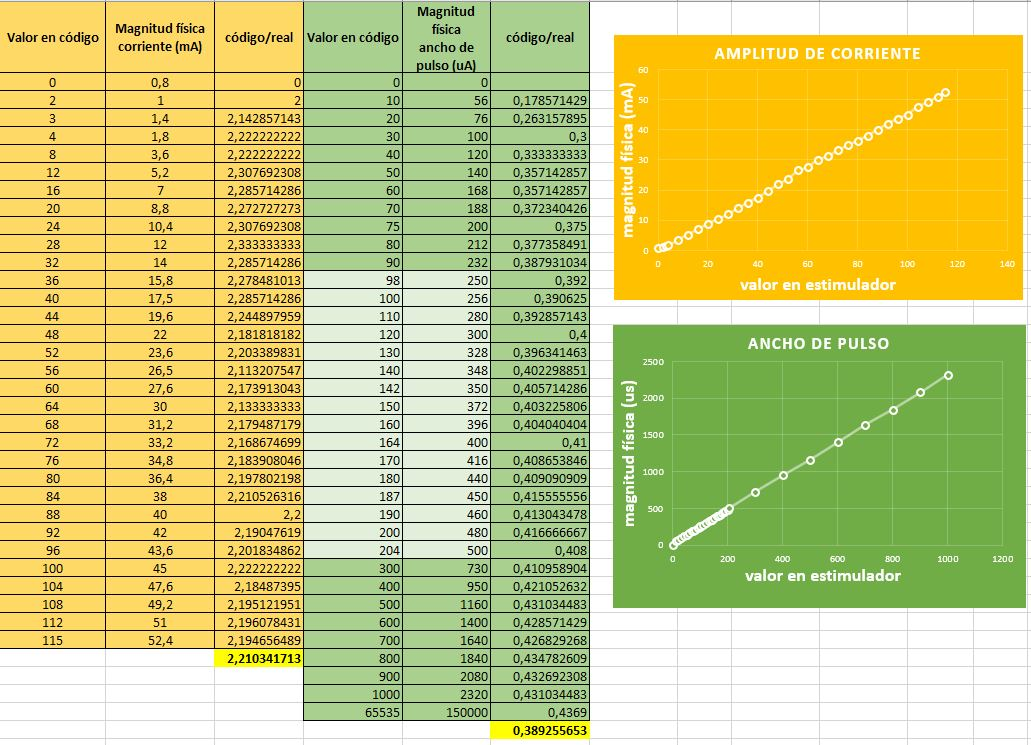
\includegraphics[scale=0.6]{factores_corriente_ancho}
  \caption{Factores de conversión de valores de amplitud de corriente y ancho de pulso manejados por el estimulador. La columna ``valor en código'' es el valor numérico que recibe mediante comandos el estimulador mientras que la columna ``magnitud física'' indica la magnitud física medida mediante un osciloscopio en el canal estiumulado. Los factores de conversión de corriente y ancho de pulso, resaltados en amarillo, se consideran constantes debido a la linealidad de la relación entre el ``valor en código'' y su ``magnitud física''.}\label{fig:factores_corriente_ancho}
\end{figure}

\begin{figure}[!htb]
\centering
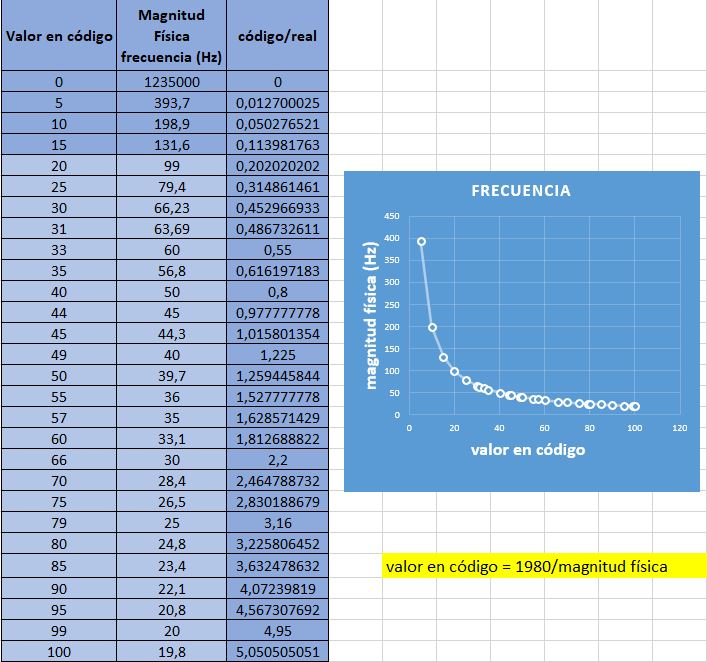
\includegraphics[scale=0.6]{factor_frecuencia}
  \caption{Factor de conversión de la frecuencia de estimulación generada por el estimulador. El ``valor en código'' es el valor numérico que el mini TEREFES recibe mediante comandos mientras que la ``magnitud física'' es la frecuencia medida en Hz en el canal estimulado. Se resalta en amarillo la función aproximada de conversión, deducida a partir del producto de los valores manejados por el estimulador y sus magnitudes físicas, pues se obtiene de forma reiterada un valor de 1980 o muy próximo.}\label{fig:factor_frecuencia}
\end{figure}

No cualquier valor de los parámetros descritos en este apartado (amplitud de corriente, ancho de pulso, frecuencia etc.) son válidos para una electroestimulación adecuada. Para el caso que concierne al proyecto con que se involucra este TFM, es decir, la rehabilitación de la marcha patológica, se consideran principalmente los miembros inferiores del cuerpo. Para estos se tienen unos rangos de valores de los mencionados parámetros mostrados a continuación:

\begin{itemize}
\item[•] \textbf{Amplitud de corriente:} La corriente inducida sobre el paciente a través de los parches adecuados tiene un valor mínimo de 0 $mA$ (no hay estimulación) y un valor máximo de 50 $mA$ (valores tan altos como el mencionado se utilizan solamente sobre músculos grandes como el cuádriceps).
\item[•] \textbf{Ancho de pulso:} el ancho de pulso oscila entre 250 y 500 $\mu s$.
\item[•] \textbf{Frecuencias inter e intra pulso:} la frecuencia de estimulación puede tomar valores tan bajos como 20$Hz$ y un valor máximo de 100$Hz$.
\end{itemize} 

Por último, se ha de tener en cuenta que la manera en la que se establecerá comunicación con los estimuladores desde el exterior es mediante la interfaz gráfica de usuario que se pretende implementar en el presente trabajo. Para ello, se integrarán en la misma las instrucciones de control ya explicadas. Además, se debe contrarrestar la conversión interna de parámetros previamante explicada para que al introducir, por ejemplo, $30mA$ como corriente de estimulación efectivamente se obtengan $30mA$ en el canal correspondiente y no otro valor.

\section{Exoesqueleto robótico}
Poner todas la especificaciones indicadas en los mails , control de posicion, par, velocidad, perfiles de movimiento etc.


\section{Sensores}
Se va a utilizar una serie de sensores para obtener más información sobre el ciclo de la marcha efectuado por el paciente así como del estado de la propia prótesis.

\subsection{Electrogoniómetros}
Para medir el ángulo de flexión de rodillas, tobillos y caderas se utilizan los electrogoniómetros desarrollados por Biometrics\cite{goniometros}. Estos sensores son capaces de medir ángulos de hasta $180\degree$ en los dos ejes perpendiculares al dispositivo, a su vez perpendiculares entre ellos, con una resolución de $0.1\degree$. Son inalámbricos y pueden trabajar hasta una distancia de $30m$ del dispositivo de recolección de datos conectado por USB a un ordenador. Cada goniómetro tiene dos canales de comunicación arrojando cada uno de ellos medidas de ángulos y demás datos referidos a uno de los dos ejes espaciales en los que efectúa dichas mediciones. La tabla \ref{fig:goniometros_specs} muestra las características de los diferentes modelos y en la figura \ref{fig:goniometros} una fotografía de los dos modelos de los que se dispone. 
\\
\\
La forma en la que se colocan estos sensores sobre el paciente se aprecia en la figura \ref{fig:goniometros_setup}. Normalmente el sensor queda fijado con cinta de doble cara a la piel pero se puede añadir cinta adhesiva alrededor de la extremidad para sujetarlo firmemente.\\

\begin{figure}[!htb]
\centering
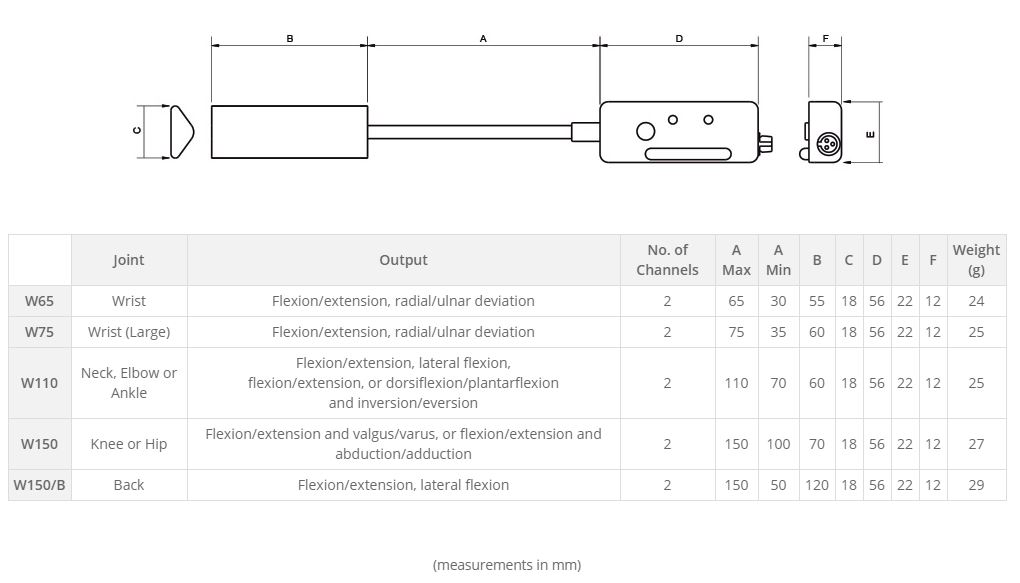
\includegraphics[scale=0.65]{goniometros_specs}
  \caption{Especificaciones de los electrogoniómetros de Biometrics\cite{goniometros}. Se dispone de dos unidades del modelo W110 y cuatro unidades del W150.}\label{fig:goniometros_specs}
\end{figure}


\begin{figure}[!htb]
\centering
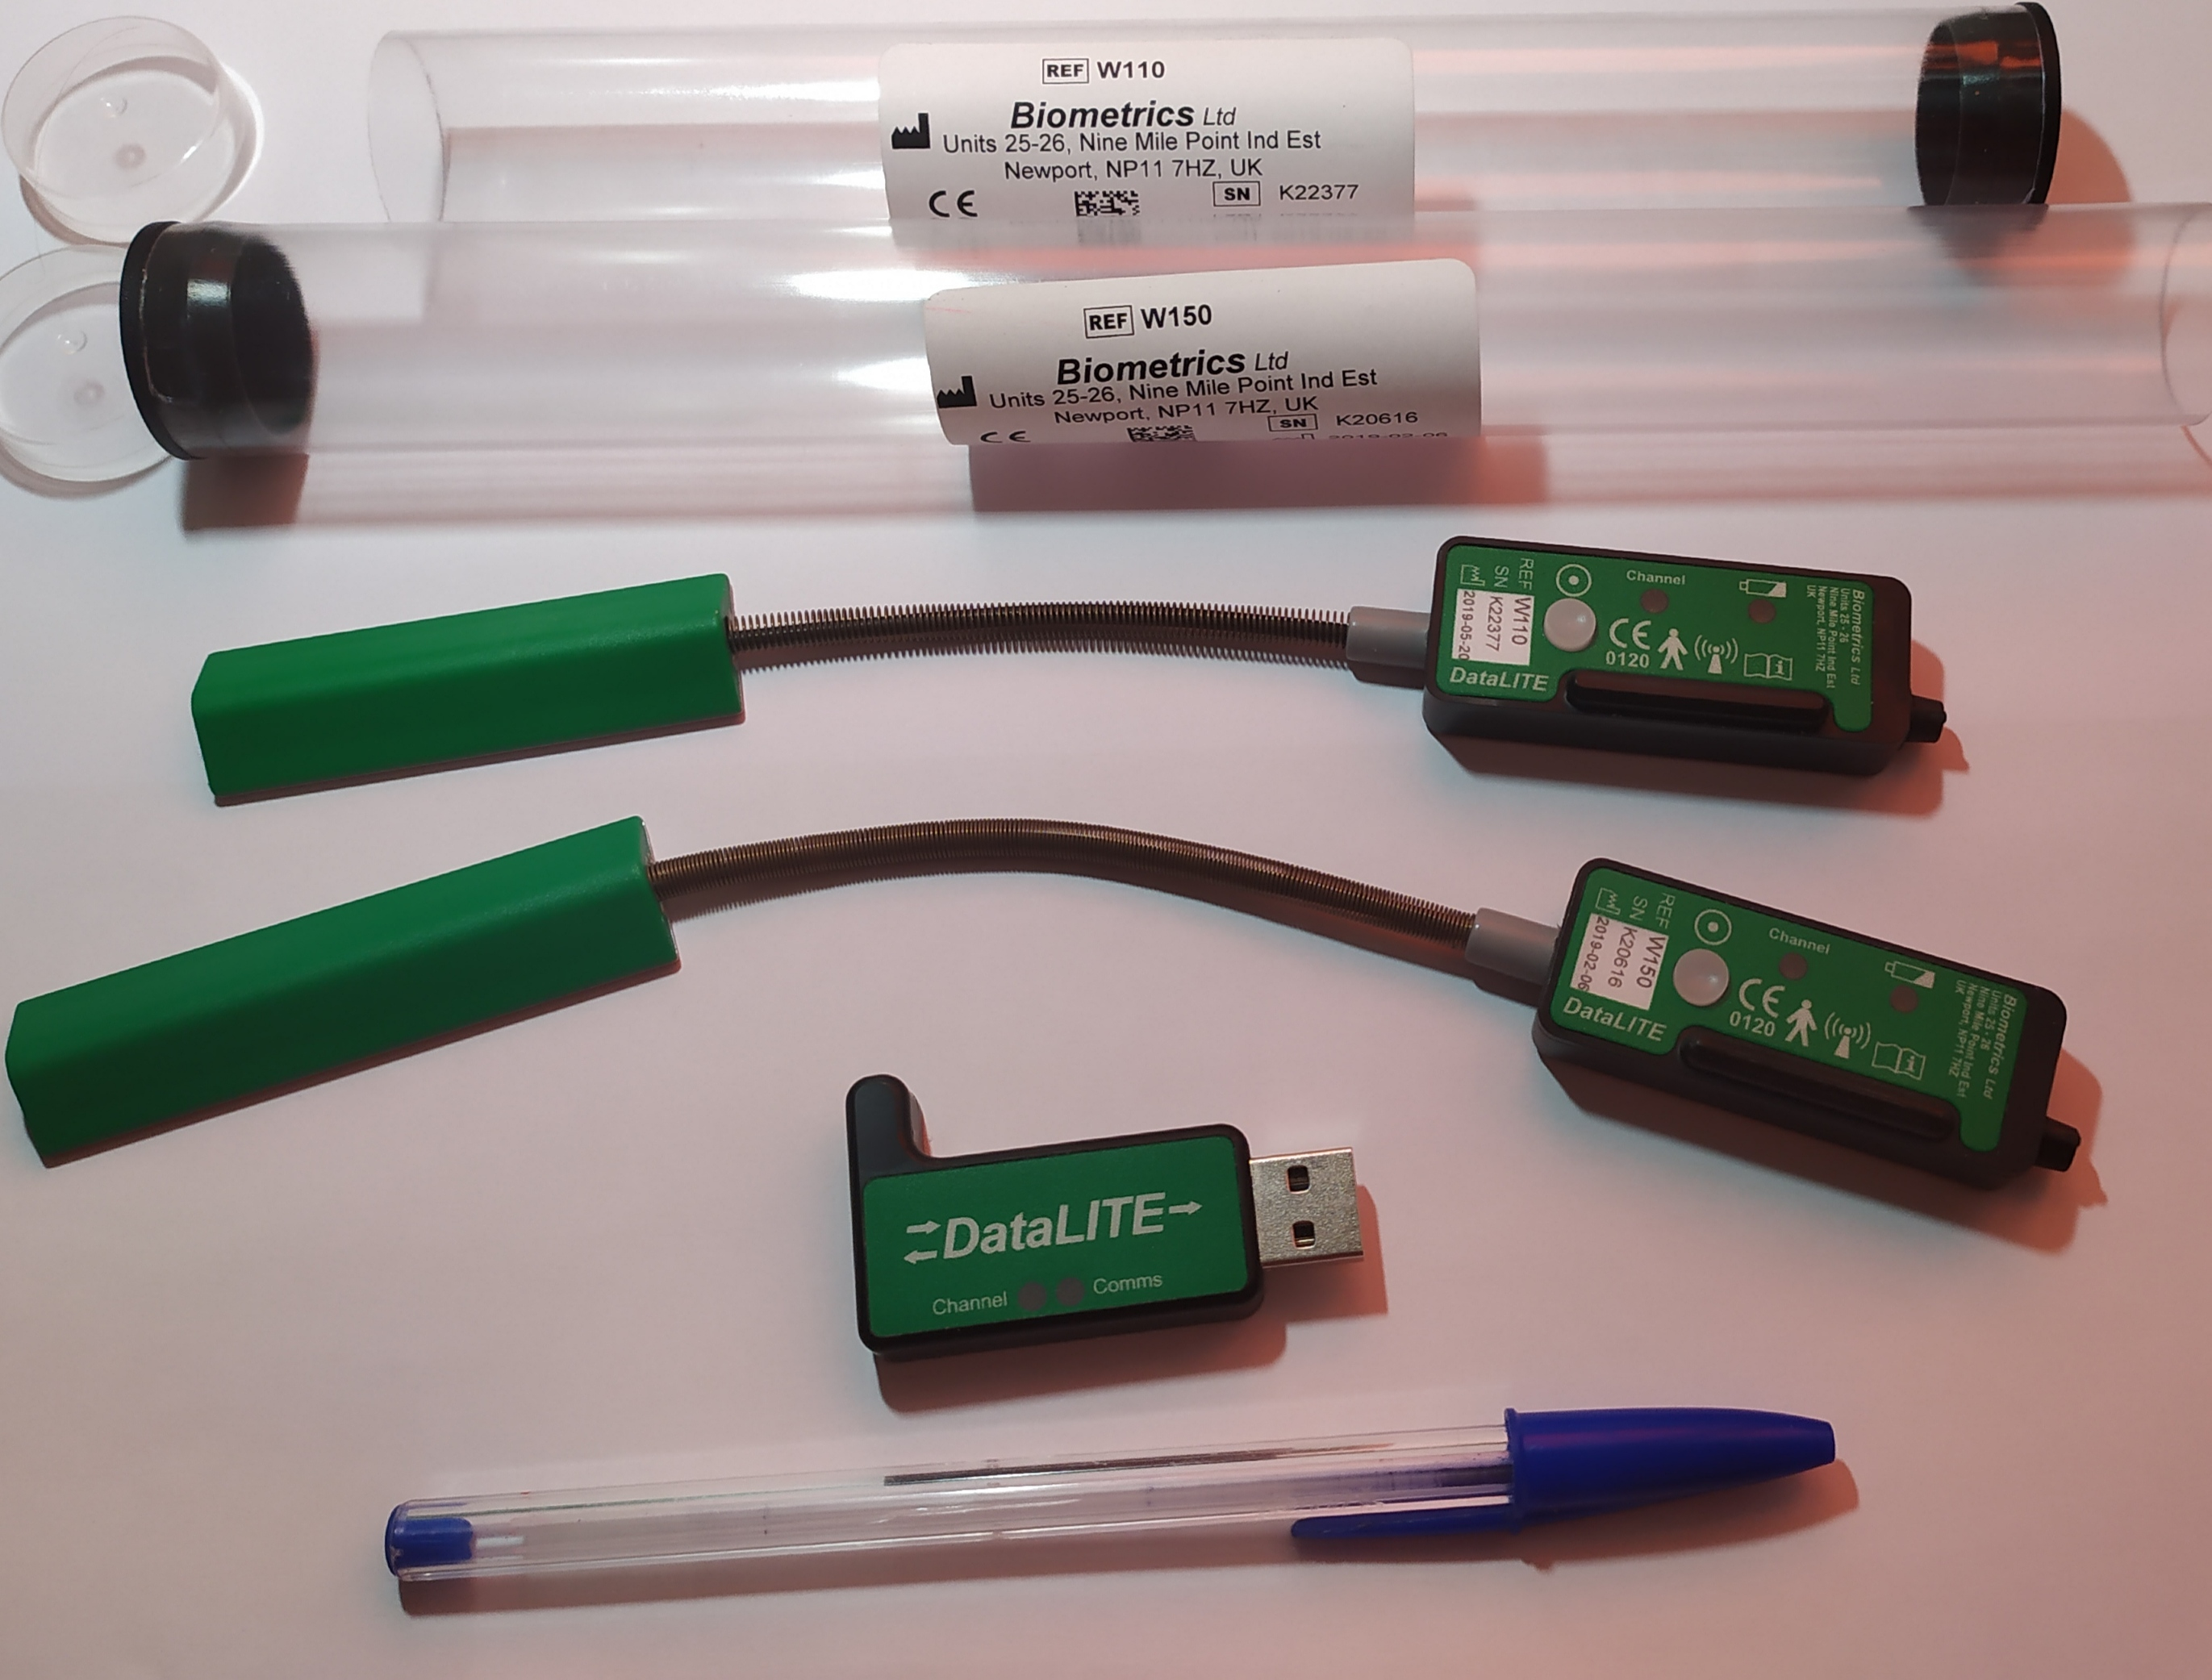
\includegraphics[scale=0.10]{goniometros}
  \caption{Electrogoniómetros W150 (grande) y W110 (pequeño) junto al receptor inalámbico de datos con conexión USB.}\label{fig:goniometros}
\end{figure}


\begin{figure}[!htb]
\centering
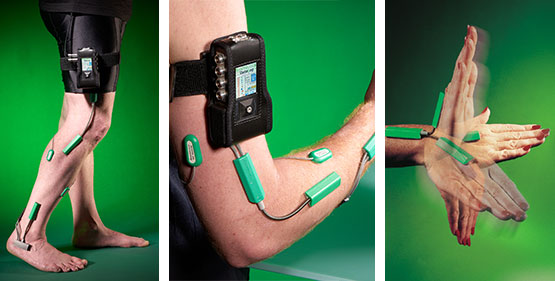
\includegraphics[scale=0.5]{goniometros_setup}
  \caption{Colocación de goniómetros sobre el paciente\cite{goniometros_setup}.}\label{fig:goniometros_setup}
\end{figure}

Junto al hardware, se dispone de la aplicación desarrollada por Biometrics para poder hacer uso de estos sensores y recolectar los datos deseados a través del receptor USB mencionado previamente. Se muestra este software en la figura \ref{fig:data_log}.\\

\begin{figure}[!htb]
\centering
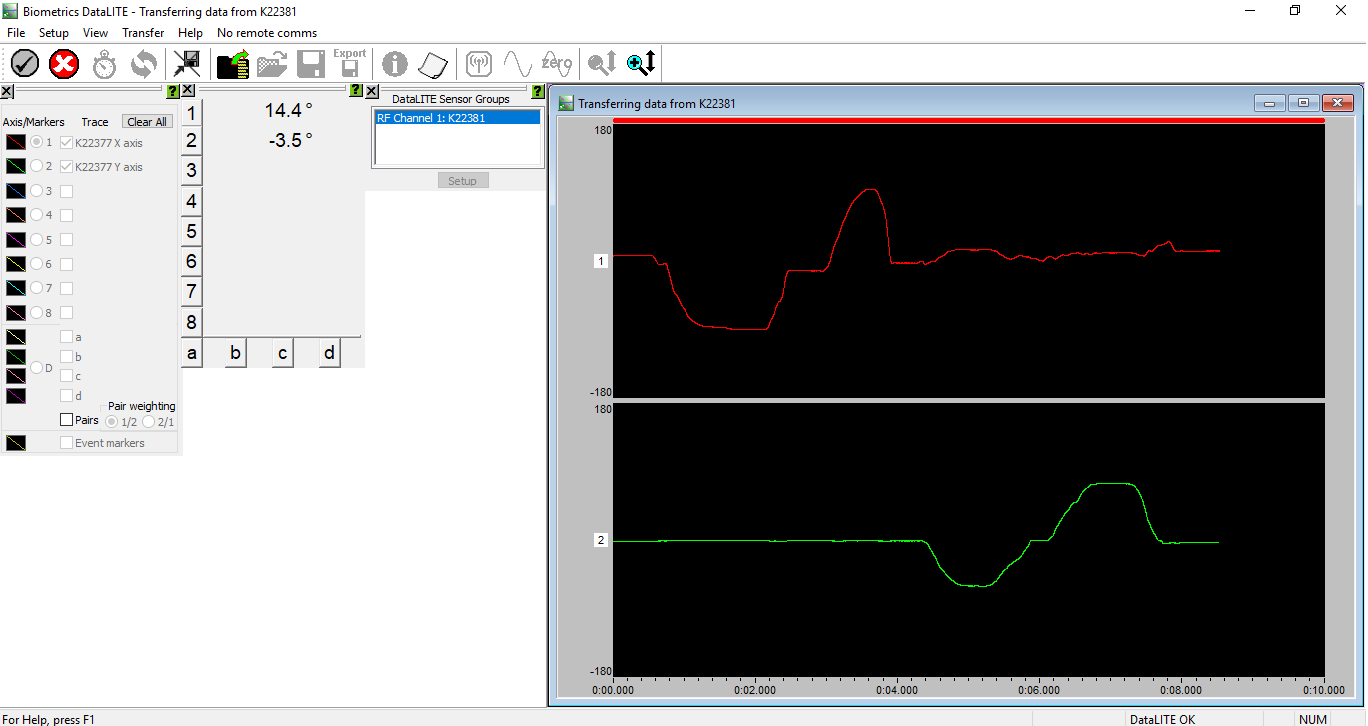
\includegraphics[scale=0.4]{data_log}
  \caption{Interfaz de Biometrics para recogida y disposición de datos de los goniómetros. Se aprecian dos gráficas, una para cada canal de un sólo goniómetro, es decir, medidas de ángulos en dos ejes perpendiculares.}\label{fig:data_log}
\end{figure}

En cuanto al funcionamiento de estos dispositivos, se diferencian dos formas de hacer uso de los mismos y obtener las mediciones de ángulos durante la ejecución del ejercicio de rehabilitación:
\begin{itemize}
\item[•] \textbf{Método directo:} implica utilizar las herramientas básicas de hardware y software ofrecidas por Biometrics. De este modo, se colocan sobre el paciente los goniómetros y se encienden pulsando el botón blanco que hay en ellos. A continuación, se conecta a un ordenador el receptor USB y se abre la aplicación de Biometrics. De acuerdo a la guía de usuario de dicha aplicación, se configura el número de goniómetros utilizados, el canal que le corresponde a cada uno y demás aspectos de configuración. Una vez dispuesto todo lo anterior, se pulsa sobre el botón de la aplicación que permite el comienzo de recepción de datos mientras se muestran en tiempo real en sus correspondientes gráficas. Cuando termina la sesión, es posible guardar en un archivo los datos de la misma.

\item[•] \textbf{Método indirecto:} implica la capacidad de recibir las mediciones de los goniómetros en una aplicación independiente y externa a Biometrics y que puede ser desarrollada por el usuario. Para ello, se debe entender cómo funciona la comunicación entre los sensores y el ordenador al que envían mediciones. Cuando se inicia en el ordenador la aplicación de Biometrics, ésta genera un espacio reservado de memoria en forma de buffer al cual le llega información de los sensores mediante el receptor USB. En el método directo, la aplicación coge estas mediciones del buffer pero en el método indirecto se pueden sacar estos datos sin necesidad de utilizar el software de Biometrics. Para ello, se dispone de unas bibliotecas de vínculos dinámicos (Dynamic-link library o DLL) que fueron entregadas por Biometrics. Estas bibliotecas contienen una serie de funciones que permiten obtener la información disponible en el buffer previamente descrito y por lo tanto hacer uso de la misma en una aplicación independiente al software de Biometrics. La figura \ref{fig:biometrics} muestra de forma esquemática el método indirecto de uso de los goniómetros.
\end{itemize}

\begin{figure}[!htb]
\centering
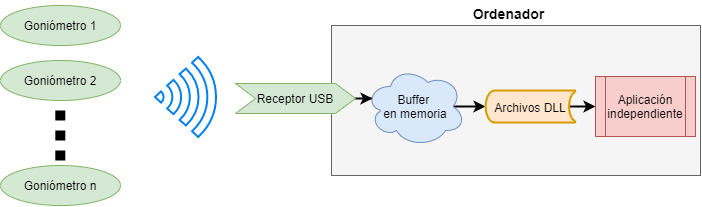
\includegraphics[scale=0.6]{biometrics}
  \caption{Proceso de transmisión de datos desde los goniómetros hasta una aplicación independiente mediante las bibliotecas aportadas por Biometrics}\label{fig:biometrics}
\end{figure}

Las bibliotecas mencionadas en el método indirecto permiten acceder a diferentes tipos de mediciones o parámetros de configuración de los goniómetros para cada uno de sus dos canales. De este modo, es posible obtener la frecuencia de muestreo así como el número de muestras disponibles en el buffer para ser leídas. Además, es posible obtener una estructura de datos que contiene un vector con las mediciones de ángulos efectuadas por el sensor. Por último, en el caso de producirse algún error, éste se refleja en los valores leídos del buffer por lo que se tiene control externo sobre lo que ocurre en los goniómetros. Es por tanto el método indirecto el ideal para hacer uso de los goniómetros en la interfaz de usuario que se pretende realizar en el presente trabajo, siendo ésta la aplicación independiente mencionada en este tipo de control. Se aprecia esta configuración en la figura \ref{fig:configuracion_actual}.\\

\begin{figure}[!htb]
\centering
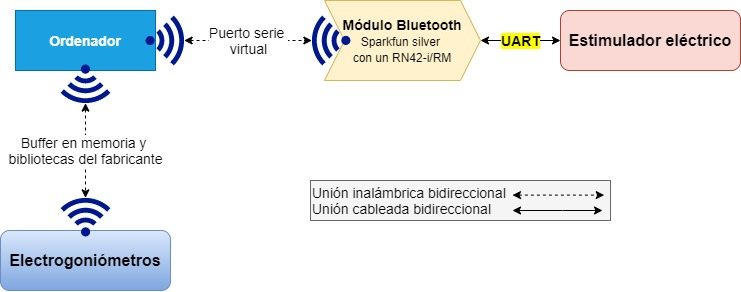
\includegraphics[scale=0.6]{configuracion_actual}
  \caption{Configuración para el control de un electroestimulador y el conjunto de goniómetros desde un ordenador.}\label{fig:configuracion_actual}
\end{figure}





